\chapter{Results}

\section{Problem Data and Result Explanation}
\begin{comment}
Existing computer code (written in C++) already exist for the TA algorithms,
including the path equilibrium method and many others.
A simple shortest path calculation algorithm is currently used by the path equilibrium method,
which runs very poorly given a small network.
\end{comment}
\marginpar{talk about\\existing\\code}

The problem data for solving the TA problems are retrieved from Transportation Network Test Problems \citep{ProblemData}.

Through out the report, Table~\ref{table:problemdata} is used to show the run time and number of iterations for solving one particular network.
In the table, the ``O-D pairs'' column gives the number of pairs of origin and destination in the network.
The ``zone'' column gives the number of traffic zones,
in some cases, the nodes in the network also include the traffic zones.
The ``Run time (seconds)'' gives is measured from executing the 
path equilibration algorithm from start to finish.
The ``Iterations'' column gives how many times the whole network
gets solved to settle the traffic flows to equilibrium.
\begin{table}[H]
    \centering
    \begin{tabular}{lrrrrrr}
        Network & Nodes & Zones & O-D pairs & Arcs & Iterations & Run Time (s) \\
        SiouxFalls    & 24   & 24  & 528   & 76   \\
        Anaheim       & 416  & 38  & 1406  & 914  \\
        Barcelona     & 1020 & 110 & 7922  & 2522 \\
        Winnipeg      & 1052 & 147 & 4344  & 2836 \\
        ChicagoSketch & 933  & 387 & 93135 & 2950 
    \end{tabular}
    \caption{Network Problem Data}
    \label{table:problemdata}
\end{table}
\marginpar{time per\\iteration?}
By examining the network problem data,
we can see that the number of O-D pairs increase
significantly respect to the number of zone nodes,
this is important because it indicates how many SPPs need to be solved for each iteration of the PE.
We can also roughly tell that these networks are very sparse,
as a complete graph (every node is connected to every other node) of 1000 nodes have 499500 arcs ($n(n-1)/2$),
and the larger networks in our problem data only have about 0.4\% to 0.6\% of arcs in a complete graph, this information is useful
when we start tuning the algorithms for solving SPP.

Most of the data does not resemble a real world transportation network, 
for example sometimes all roads have the same speed limit, road type and capacity.

In this report, all problem data are solved on a Intel i5 1.78GHz CPU computer with 4GB RAM, which runs the Ubuntu 12.04 Linux operating system.
And the code is compiled with the g++ compiler with the -O3 optimisation flag (i.e.\ optimise for speed).

The accuracy of all results are checked by comparing the traffic flows from the traffic assignment output,
as well as the final shortest path for every O-D pairs.
\marginpar{CPU\\param}

\begin{comment}
The existing shortest path algorithm in the traffic assignment code is called the label correcting algorithm.
The code is adapted from \citep{Sheffi}, 
\end{comment}

\begin{table}
    \centering
    \begin{tabular}{lrrrrrr}
        Network & Nodes & Zones & O-D Pairs & Arcs  & Iterations  & Run Time (s) \\ 
        SiouxFalls    & 24   & 24  & 528   & 76      & 69         & $ 0.25 $     \\ 
        Anaheim       & 416  & 38  & 1406  & 914     & 10         & $ 1.20  $     \\
        Barcelona     & 1020 & 110 & 7922  & 2522    & 28         & $ 60.00   $     \\
        Winnipeg      & 1052 & 147 & 4344  & 2836    & 129        & $ 190.00  $     \\
        ChicagoSketch & 933  & 387 & 93135 & 2950    & 25         & $ 500.00  $    
    \end{tabular}
    \caption{One Source Label Correcting Algorithm Result}
\end{table}

Using the standard C++ standard template library (STL) priority queue (implemented as a Heap tree) using std::vector as the underlying storage,
the following results are generated.
\begin{table}
    \centering
    \begin{tabular}{lrrrrrrr}
        Network & Nodes & Zones & O-D Pairs & Arcs  & Iterations & Run Time (s) \\
        SiouxFalls    & 24   & 24  & 528   & 76     & 64         & $ 0.24 $     \\
        Anaheim       & 416  & 38  & 1406  & 914    & 10         & $ 1.20 $     \\
        Barcelona     & 1020 & 110 & 7922  & 2522   & 27         & $ 43.00 $    \\
        Winnipeg      & 1052 & 147 & 4344  & 2836   & 129        & $ 137.00 $   \\
        ChicagoSketch & 933  & 387 & 93135 & 2950   & 25         & $ 541.00 $  
    \end{tabular}
    \caption{C++ STL One-Source Label Setting Algorithm Result}
\end{table}


The following table shows the result for point to point Dijkstra's algorithm.
\begin{table}[H]
    \centering
    \begin{tabular}{lrrrrrr}
        Network & Nodes & Zones & O-D Pairs & Arcs  & Iterations & Run Time (s) \\
        SiouxFalls    & 24   & 24  & 528   & 76     & 64         & $ 0.15 $     \\
        Anaheim       & 416  & 38  & 1406  & 914    & 10         & $ 0.67 $     \\
        Barcelona     & 1020 & 110 & 7922  & 2522   & 27         & $ 27.71$     \\
        Winnipeg      & 1052 & 147 & 4344  & 2836   & 129        & $ 70.00  $   \\
        ChicagoSketch & 933  & 387 & 93135 & 2950   & 25         & $ 204.00  $ 
    \end{tabular}
    \caption{Point to Point Label Setting Algorithm (Dijkstra) Result}
\end{table}

The following table shows the run time and iterations for all the networks.
\begin{table}[H]
    \centering
    \begin{tabular}{lrrrrrrr}
        Network       & Iterations & Binary & Ternary & Binomial & Fibonacci & Pairing & Skew \\
        SiouxFalls    & 85         & 0.17 & 0.17 & 0.29 & 0.18 & 0.17 & 0.16                  \\
        Anaheim       & 10         & 0.88 & 0.81 & 2.12  & 1.05 & 1.02 & 0.83                 \\
        Barcelona     & 27         & 34.00 & 33.00 & 85.00 & 46.00 & 44.00 & 34.00            \\
        Winnipeg      & 128        & 83.00 & 86.00 & 202.00 & 107.00 & 97.00 & 83.00          \\
        ChicagoSketch & 26         & 233.00 & 229.00 & 472.00 & 264.00 & 231.00 & 209.00      
    \end{tabular}
    \caption{Point to Point C++ Boost Label Setting Algorithm (Dijkstra) Result}
    \label{table:dijkstraresult}
\end{table}

Results:
\begin{table}[H]
    \centering
    \begin{tabular}{lrr rrr rrr}
        Network        & Iterations & STL & Binary & Ternary & Binomial & Fibonacci & Pairing & Skew \\
        SiouxFalls     & 85           & 0.16 & 0.14 & 0.16 & 0.22  & 0.22  & 0.14  & 0.14            \\
        Anaheim        & 10           & 0.15 & 0.19 & 0.19 & 0.33  & 0.22  & 0.18  & 0.17            \\
        Barcelona      & 27           & 5.44 & 6.53 & 6.54 & 11.45 & 7.62  & 6.56  & 6.10            \\
        Winnipeg       & 128          & 19.49& 24.34& 24.86& 44.41 & 27.93 & 24.23 & 21.85           \\ 
        ChicagoSketch  & 26           & 38.92& 46.00   & 44.00   & 78.02 & 53.28 & 45.10 & 42.90       
    \end{tabular}
    \caption{A* Algorithm Result}
    \label{table:astarresult}
\end{table}


\begin{figure}
    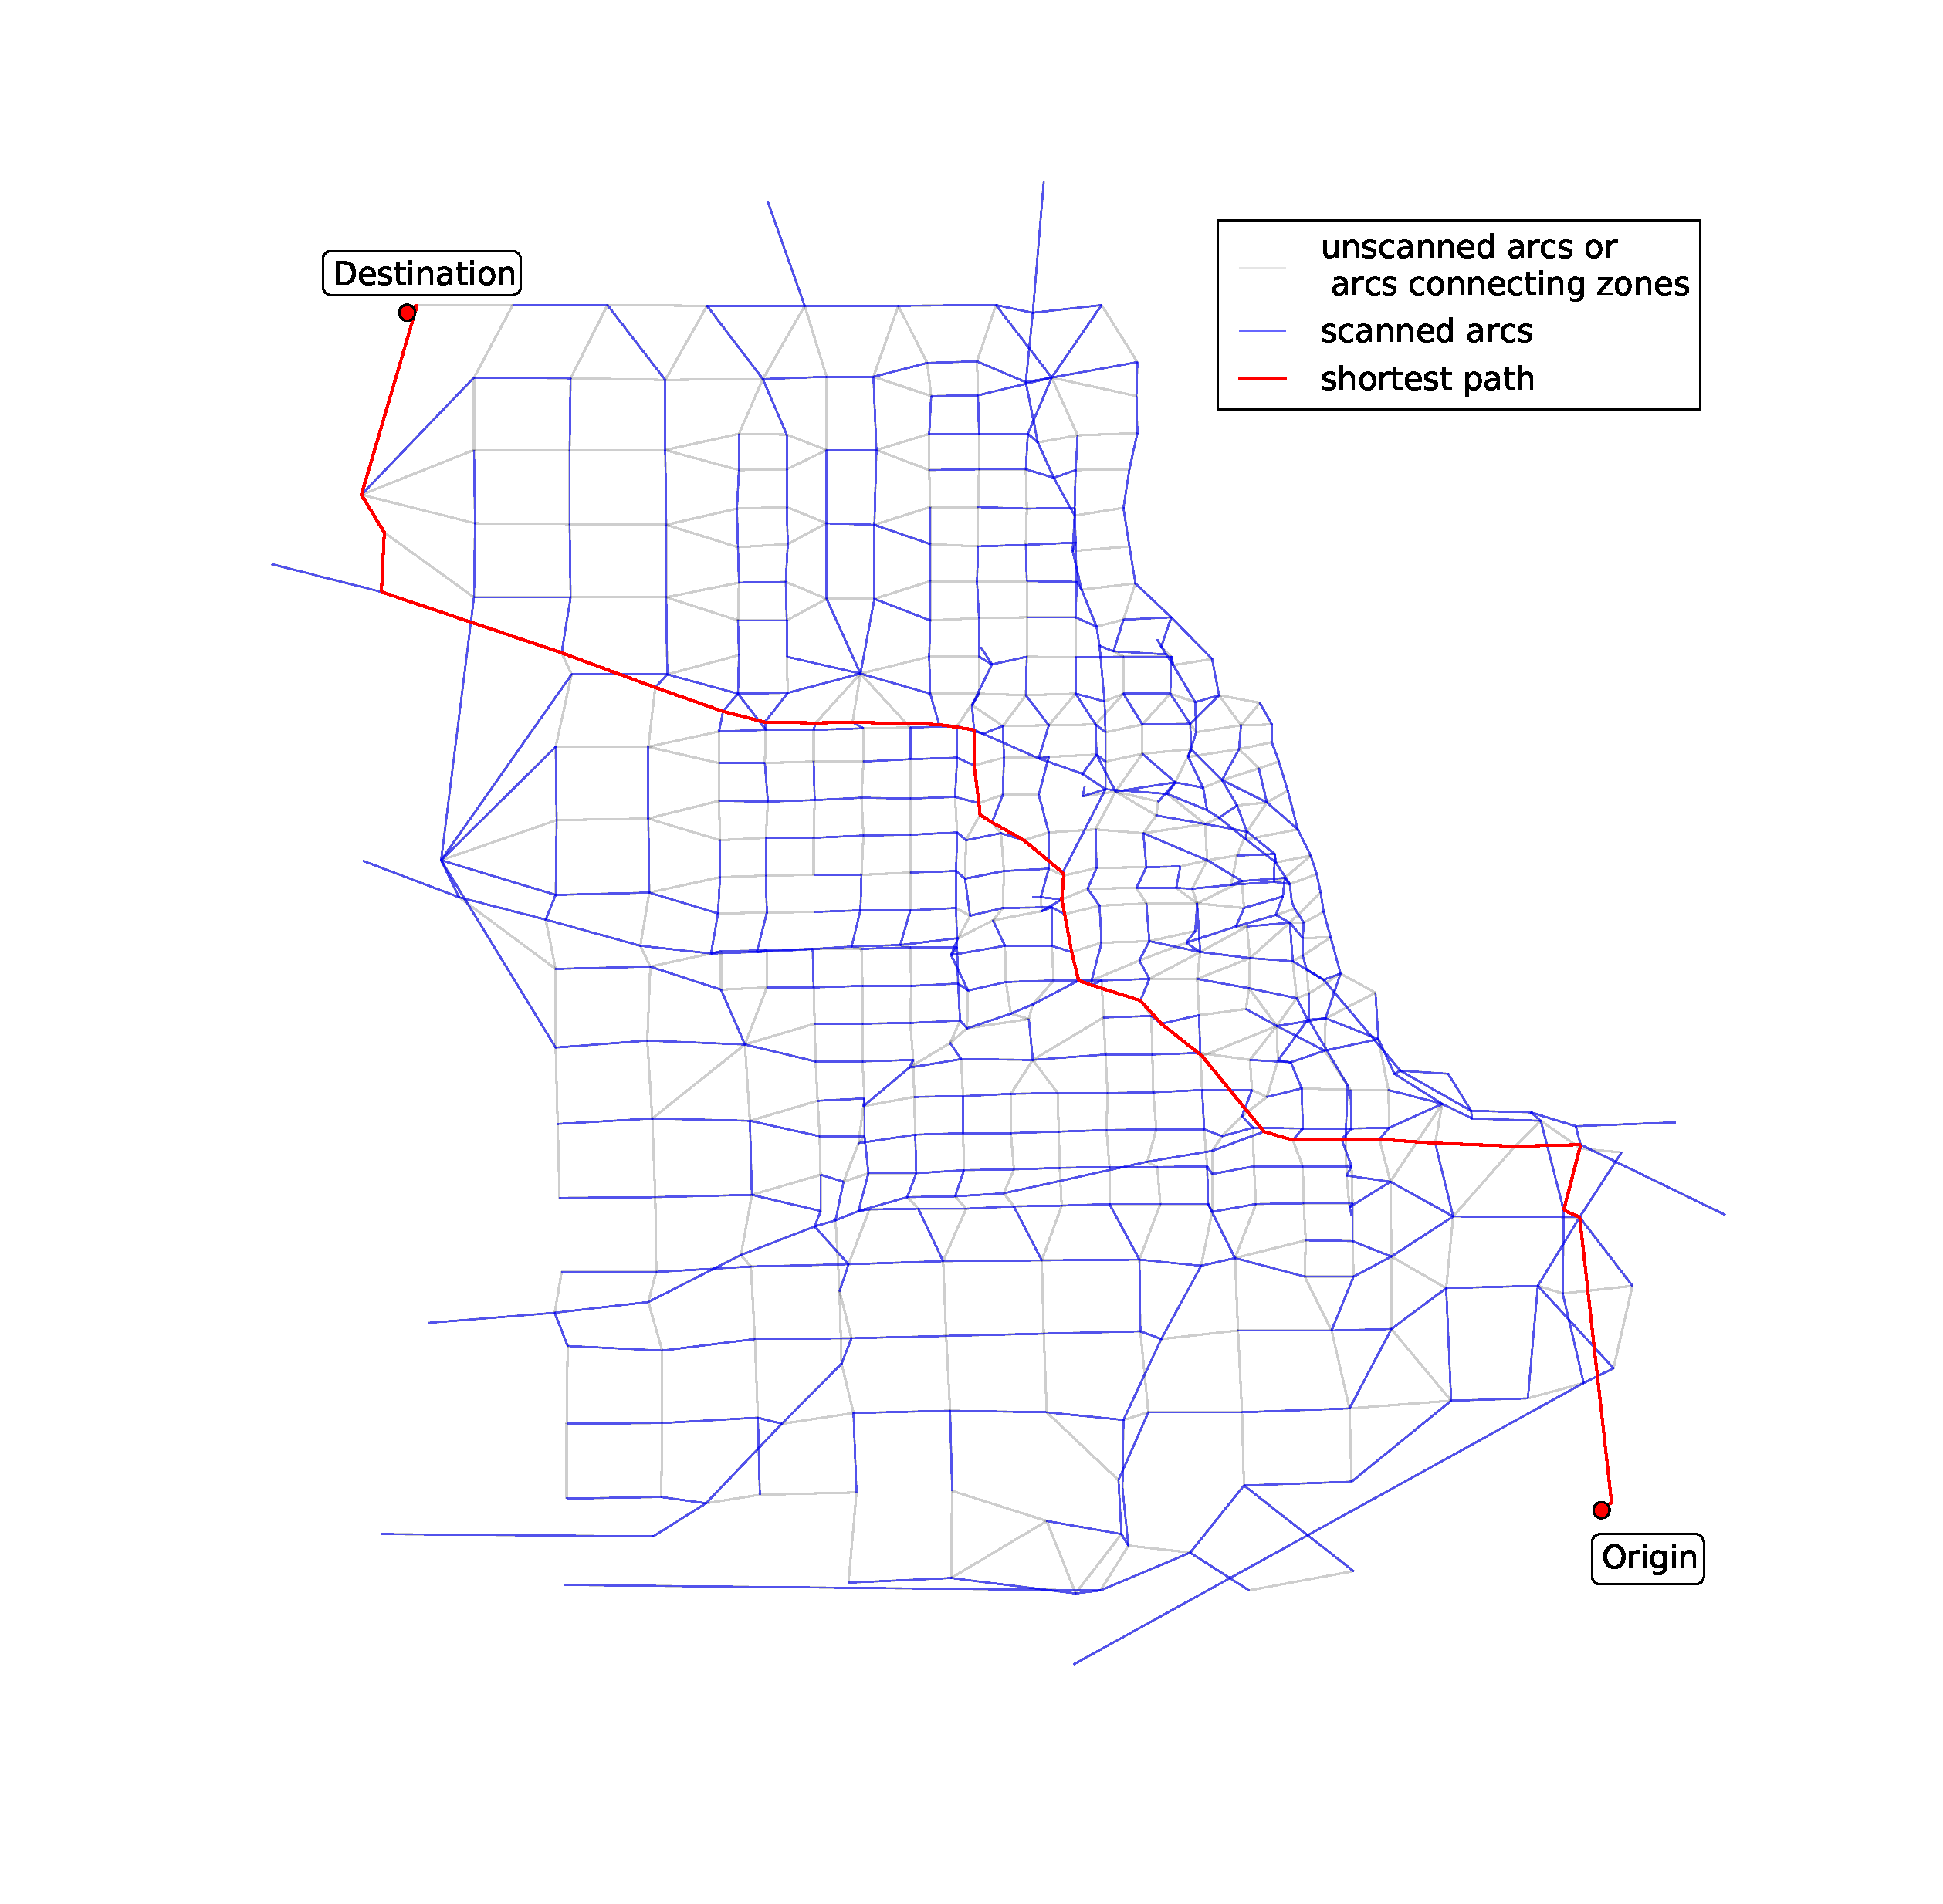
\includegraphics[width=\textwidth,trim=120px 120px 48px 120px,clip]{img/chicago_dijkstra}
    \caption{Dijkstra Path Tree for ChicagoSketch network}
    \label{fig:astarchicago}
\end{figure}

\begin{figure}
    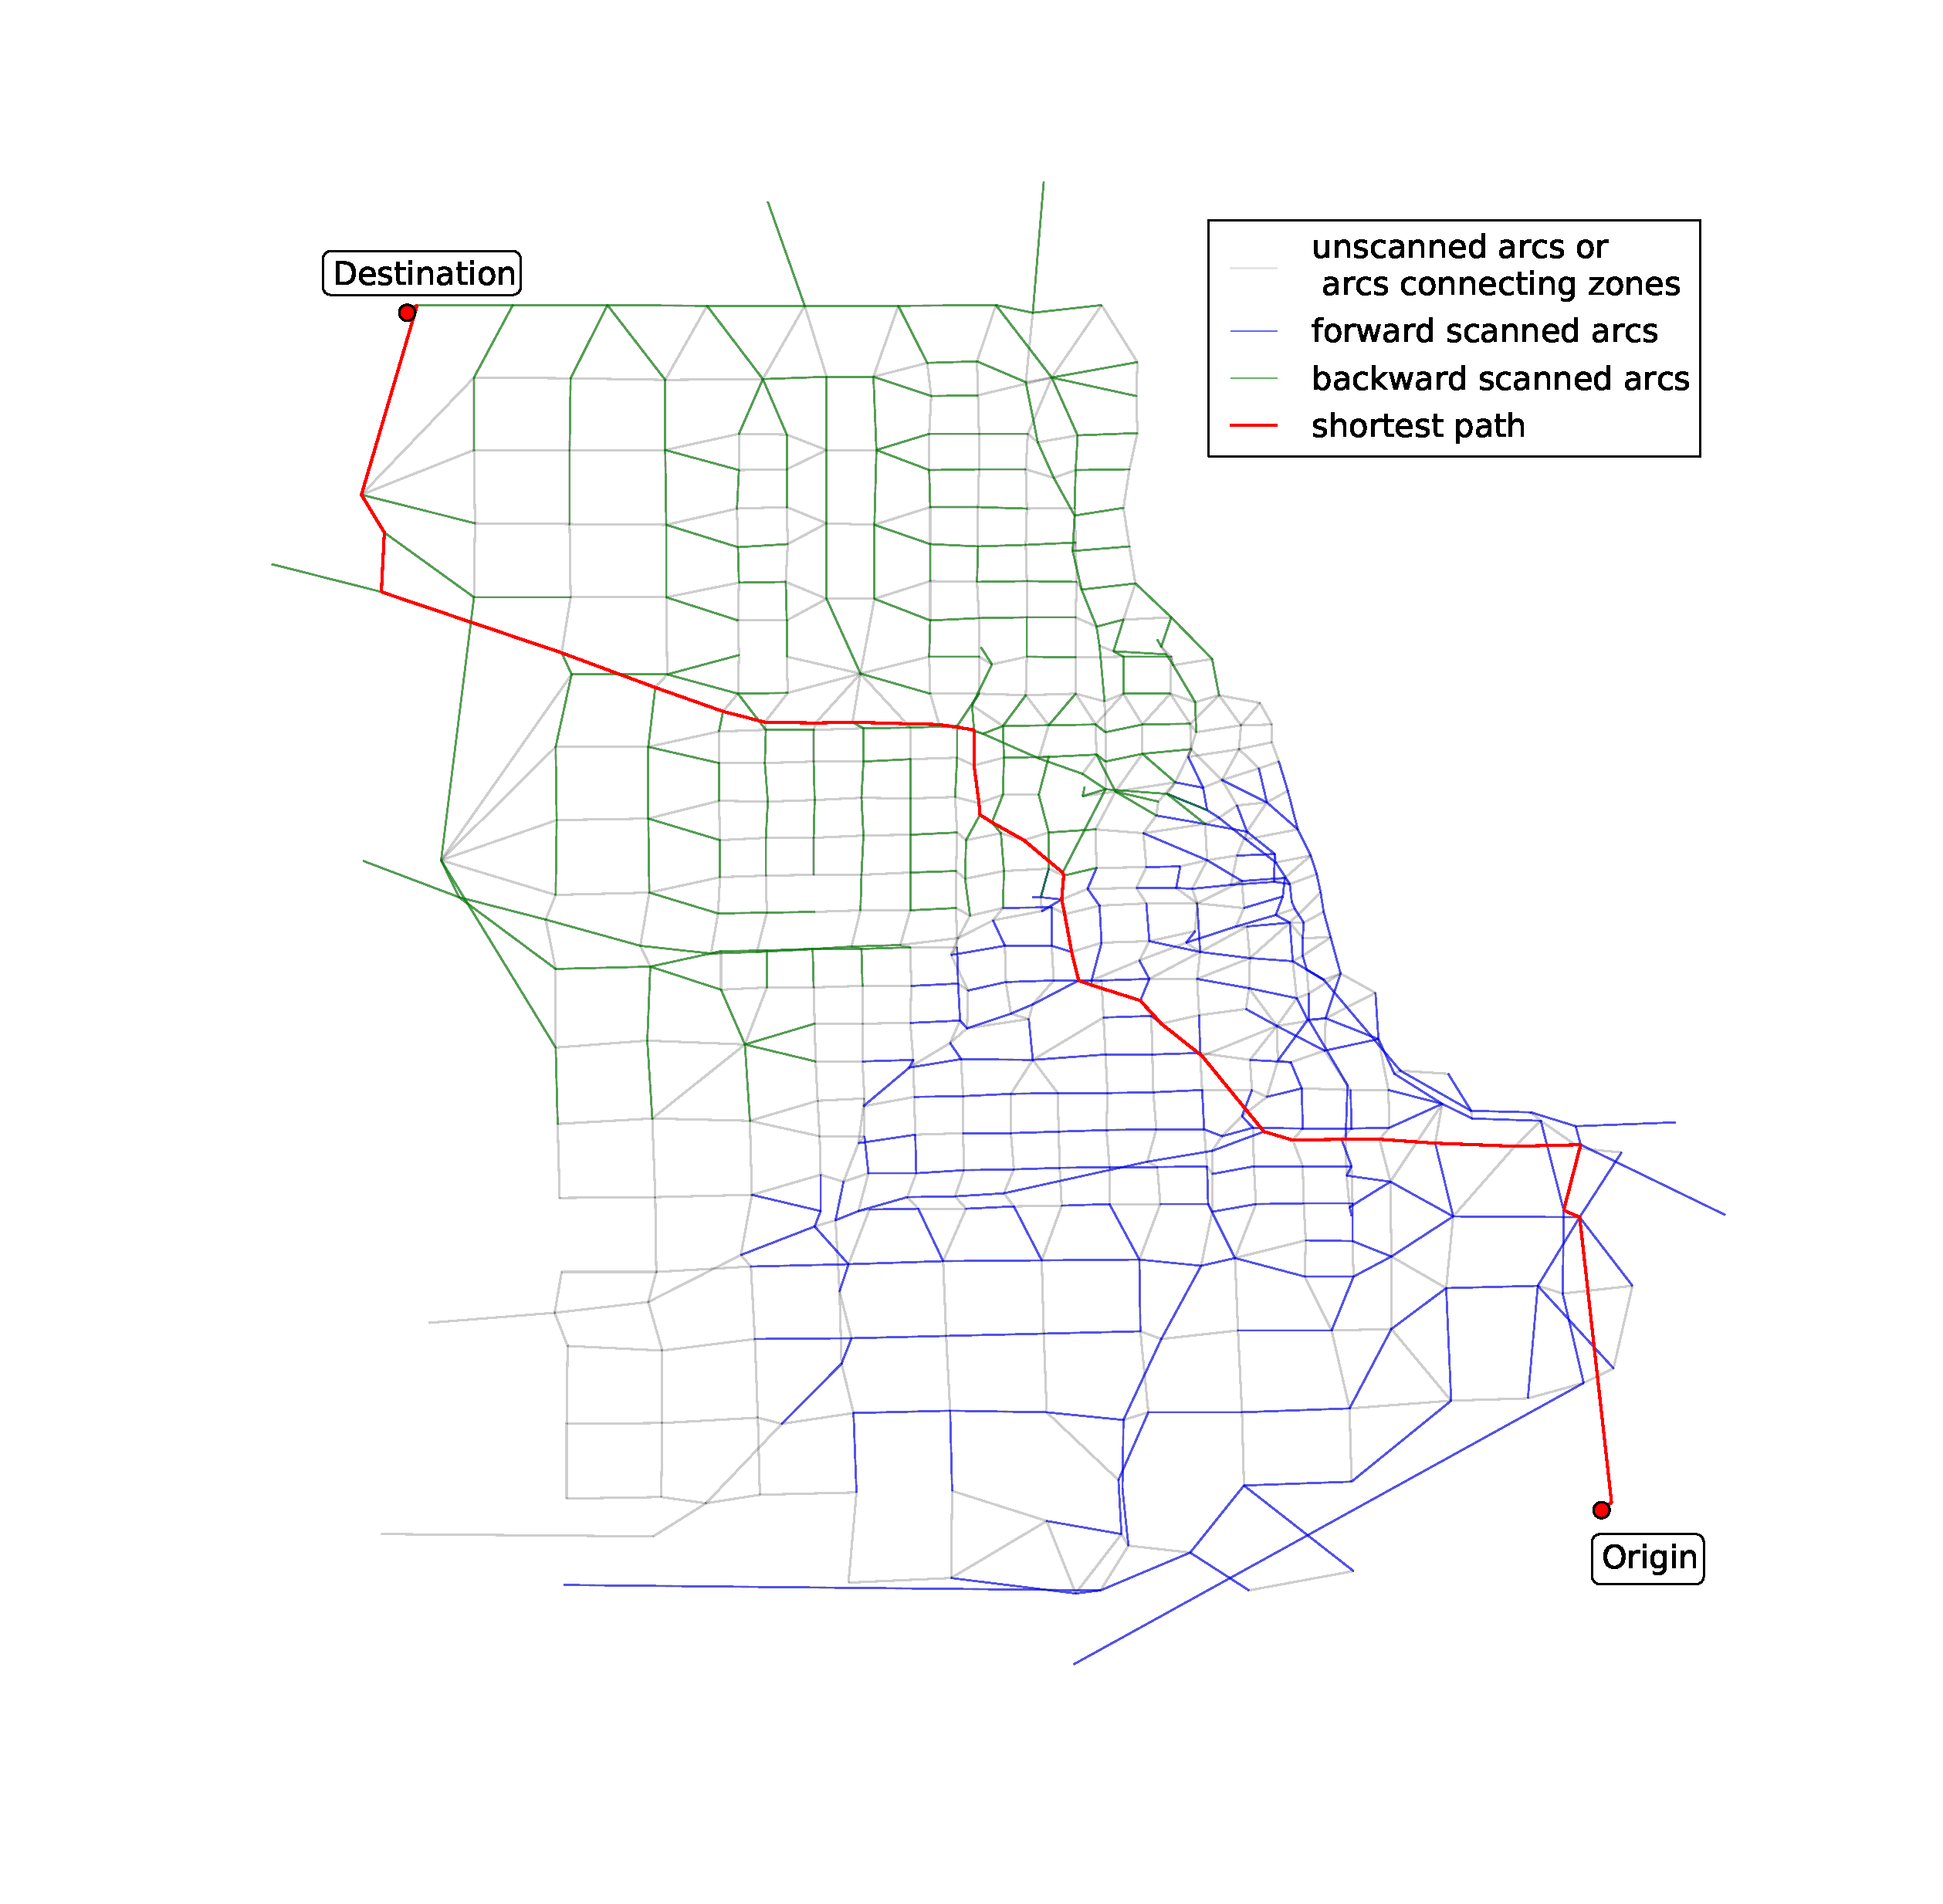
\includegraphics[width=\textwidth,trim=120px 120px 48px 120px,clip]{img/chicago_bidirect}
    \caption{Bidirectional Dijkstra Shortest Path Tree for ChicagoSketch network}
    \label{fig:astarchicago}
\end{figure}

\begin{figure}
    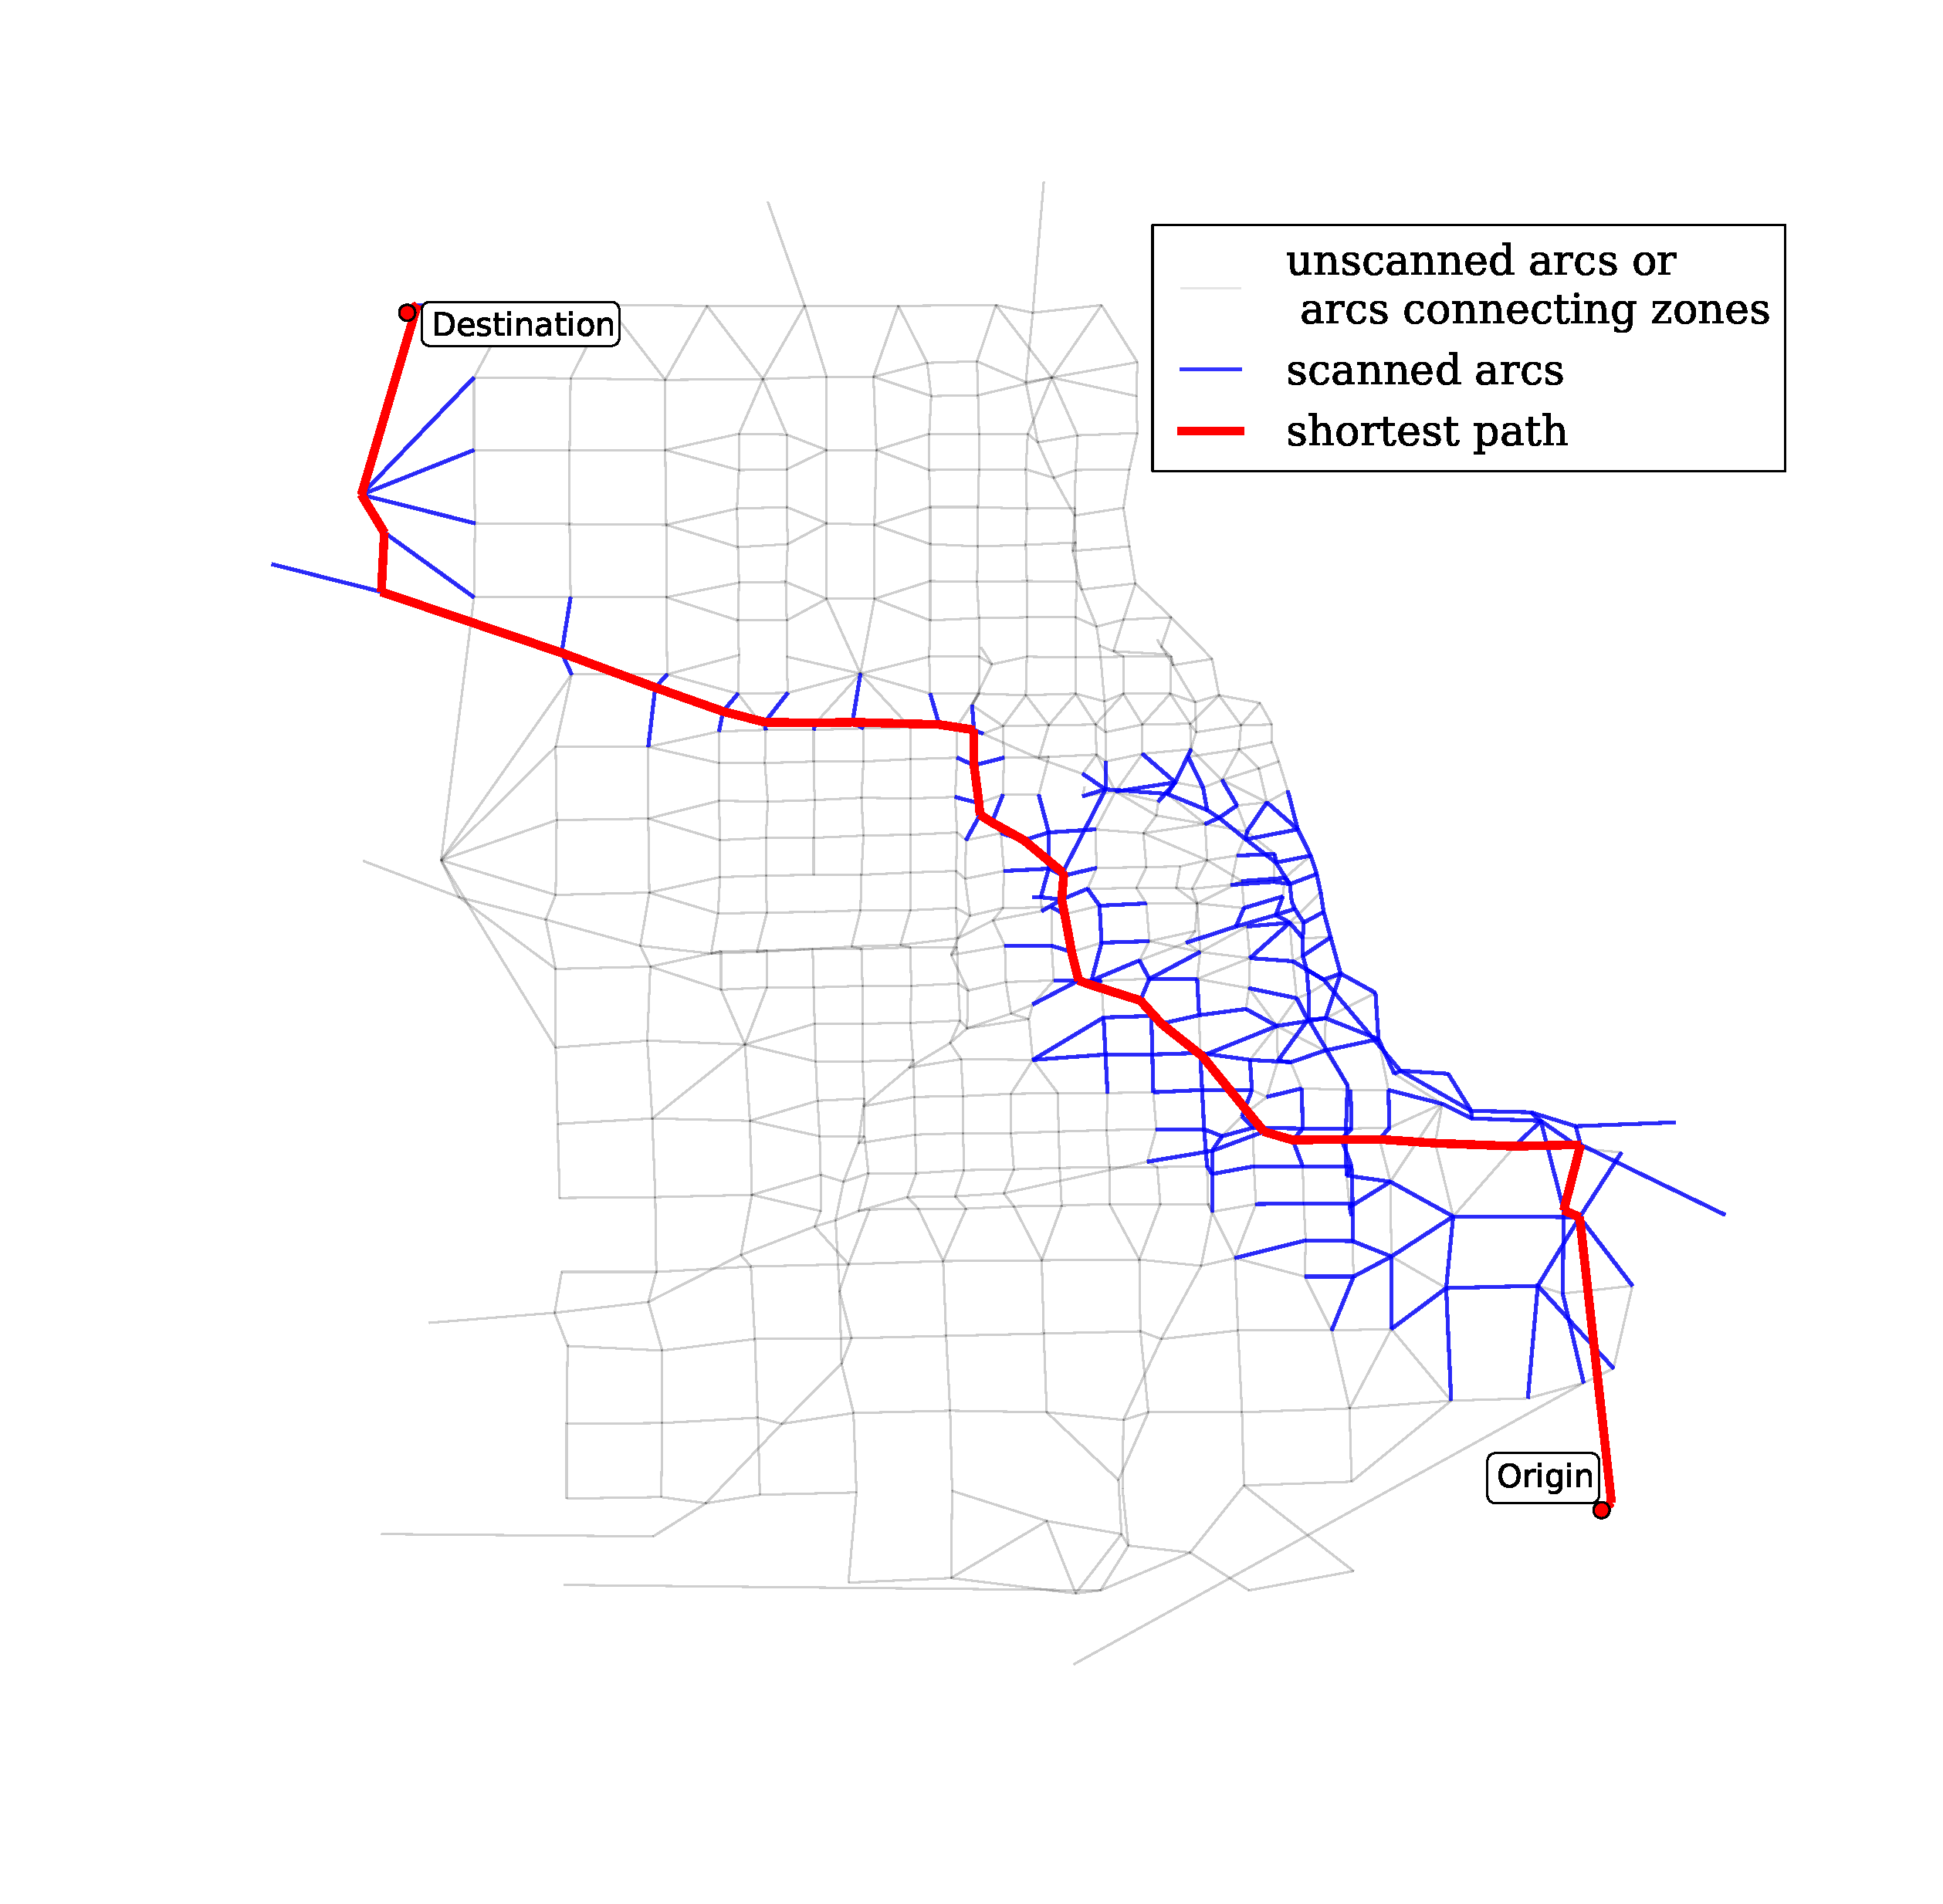
\includegraphics[width=\textwidth,trim=120px 120px 48px 120px,clip]{img/chicago_astar}
    \caption{A* Shortest Path Tree for ChicagoSketch network}
    \label{fig:astarchicago}
\end{figure}
